\documentclass[11pt,a4paper,oneside]{article}
\usepackage[utf8]{inputenc}
\usepackage[T1]{fontenc}
\usepackage[french]{babel}
\usepackage{lmodern}
\usepackage{microtype}
\usepackage[a4paper,margin=2.25cm,headheight=15pt,footskip=28pt]{geometry}
\usepackage{amsmath,amssymb,amsthm,mathtools}
\usepackage{booktabs,tabularx,array}
\usepackage[dvipsnames]{xcolor}
\usepackage{tikz}
\usepackage{graphicx}
\usetikzlibrary{arrows.meta,calc,intersections,angles,quotes,patterns,positioning,decorations.pathreplacing}
\usepackage{fancyhdr}
\usepackage{hyperref}
\usepackage{enumitem}

\definecolor{Forest}{HTML}{1D5B4A}
\definecolor{Ink}{HTML}{16211D}
\definecolor{Mist}{HTML}{EAF0EC}
\definecolor{Muted}{HTML}{5B6862}
\hypersetup{colorlinks=true,linkcolor=Forest,urlcolor=Forest,citecolor=Forest,pdftitle={Curiosité mathématique},pdfauthor={Germain-Junior TWAMBA}}
\urlstyle{same}
\setlength{\parskip}{0.45em}
\setlength{\parindent}{0pt}
\setlist[enumerate]{leftmargin=2em,itemsep=0.25em,topsep=0.3em}
\setlist[itemize]{leftmargin=1.5em,itemsep=0.2em,topsep=0.3em}
\pagestyle{fancy}
\fancyhf{}
\fancyhead[L]{\small\textcolor{Muted}{Curiosités mathématiques}}
\fancyhead[R]{\small\textcolor{Muted}{Club des Divergents}}
\fancyfoot[C]{\small\textcolor{Muted}{\thepage}}
\renewcommand{\headrulewidth}{0.35pt}
\renewcommand{\footrulewidth}{0pt}
\newtheorem{theoreme}{Théorème}[section]
\newtheorem{proposition}[theoreme]{Proposition}
\newtheorem{lemme}[theoreme]{Lemme}
\theoremstyle{definition}
\newtheorem{definition}[theoreme]{Définition}
\newtheorem{exemple}[theoreme]{Exemple}
\newcommand{\titreDossier}[3]{%
  \begin{titlepage}\centering\vspace*{1.3cm}
  {\large\scshape\textcolor{Forest}{Club des Divergents \textbullet{} Goma, RDC}}\\[1.5cm]
  {\color{Forest}\rule{0.82\textwidth}{1.2pt}}\\[0.8cm]
  {\Huge\bfseries\sffamily\color{Ink}#1\par}\vspace{0.7cm}
  {\Large\color{Forest}#2\par}\vspace{1.2cm}
  {\large\color{Muted}Dossier de curiosité mathématique\par}
  \vfill
  \begin{minipage}{0.78\textwidth}\centering\large #3\end{minipage}
  \vfill
  {\color{Forest}\rule{0.82\textwidth}{1.2pt}}\\[0.45cm]
  {\large Germain-Junior TWAMBA\par}
  {\normalsize 13 novembre 2026\par}
  \end{titlepage}}
\newcommand{\sourceweb}[2]{\item \textbf{#1.} \url{#2}}
\newcommand{\idee}[1]{\begin{quote}\small\colorbox{Mist}{\parbox{0.94\linewidth}{\textbf{Idée à retenir.} #1}}\end{quote}}
\newcommand{\demonstration}{\par\smallskip\noindent\textbf{Démonstration.}\ }
\newcommand{\finpreuve}{\hfill$\square$\par}

\begin{document}
\titreDossier{Le théorème de Pascal}{Hexagone inscrit, conique et droite de Pascal}{
Un résultat projectif étonnant : six points choisis sur une même conique engendrent, par les intersections de côtés opposés, trois points toujours alignés. Ce dossier construit l'énoncé, le cadre projectif, une preuve analytique complète et un exemple calculé.}

\section*{Pourquoi six points donnent-ils une droite ?}
Un cercle paraît d'abord être un objet de métrique : on parle de centre, de rayon et de distance. Le théorème de Pascal révèle une autre structure. Si l'on ne retient que les incidences entre points et droites, tous les cercles et toutes les coniques non dégénérées ont le même comportement. Six points d'une conique suffisent à faire apparaître une nouvelle droite.

\begin{theoreme}[Pascal]
Soient $A,B,C,A',B',C'$ six points distincts d'une conique non dégénérée du plan projectif. Formons les trois intersections
\[
 P=AB'\cap A'B,\qquad Q=BC'\cap B'C,\qquad R=CA'\cap C'A.
\]
Alors $P,Q,R$ sont alignés. La droite qui les contient s'appelle la \emph{droite de Pascal} de la configuration.
\end{theoreme}

Les lettres indiquent un appariement précis des six côtés de l'hexagone croisé. On peut lire le parcours des sommets comme $A,B',C,A',B,C'$. Les trois couples de côtés opposés sont alors ceux qui définissent $P,Q,R$. La formulation est valable pour une ellipse, une parabole ou une hyperbole. Dans le plan affine, deux côtés parallèles n'ont pas d'intersection visible ; dans le plan projectif, ils se rencontrent en un point à l'infini et l'énoncé reste uniforme.

\begin{figure}[htbp]
\centering
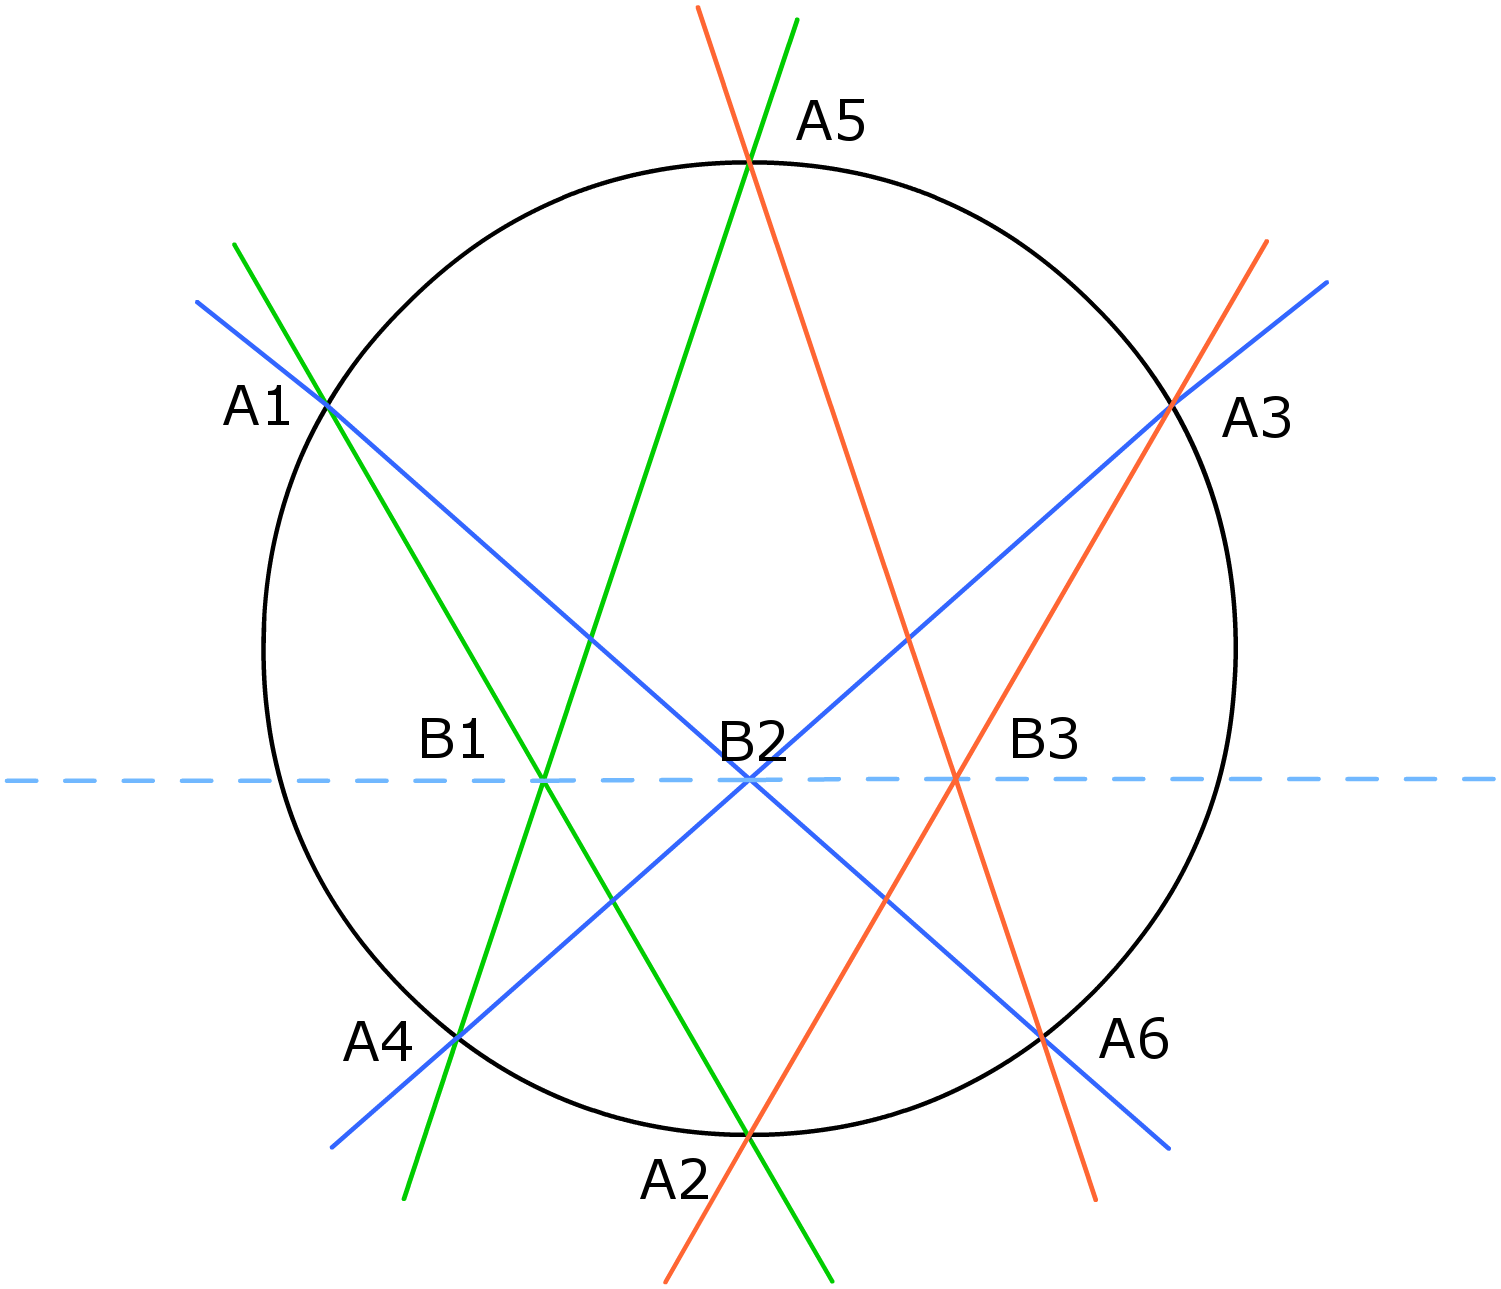
\includegraphics[width=0.66\linewidth]{images/pascal-theorem-white.png}
\caption{Une configuration du théorème de Pascal : les intersections des paires de côtés opposés sont alignées. Illustration de .jhc., diffusée dans le domaine public sur Wikimedia Commons ; fond transparent aplati sur blanc pour l'impression. Voir la \href{https://commons.wikimedia.org/wiki/File:Pascal\%27s_theorem.png}{notice de l'image}.}
\end{figure}

\section{Un mot d'histoire}
En 1640, à seize ans, Blaise Pascal fait imprimer un court \emph{Essay pour les coniques}, une affiche d'environ 35 sur 43~cm tirée à une cinquantaine d'exemplaires. Il y énonce ce résultat sans le démontrer. Le théorème de Pappus (IVe siècle) en est le cas dégénéré où la conique est formée de deux droites. Le dossier ci-dessous ne suit pas la démonstration de Pascal : il en donne une preuve analytique moderne, entièrement vérifiable.

\section{Le langage projectif nécessaire}
Un point projectif est une classe de triplets non nuls $(x,y,z)$, notée $[x:y:z]$, où deux triplets représentent le même point lorsqu'ils diffèrent par un facteur non nul. La droite d'équation $ux+vy+wz=0$ est représentée par le triplet de coefficients $[u:v:w]$. L'intersection de deux droites se calcule par produit vectoriel de leurs triplets ; la droite passant par deux points se calcule de la même façon.

Cette écriture traite les points à l'infini sans ajouter de cas particuliers. Dans la carte affine $z=1$, un point ordinaire $[x:y:1]$ a pour coordonnées $(x,y)$. Les points $[x:y:0]$ représentent les directions. Par exemple, les droites parallèles $y=0$ et $y=1$ n'ont aucune intersection dans la carte affine, mais leurs représentantes projectives se coupent en $[1:0:0]$.

Une transformation projective est induite par une matrice inversible $3\times3$. Elle envoie droites sur droites et conserve l'incidence, l'alignement et les coniques. Elle ne conserve pas en général les longueurs ni les angles. C'est pourquoi Pascal appartient naturellement à la géométrie projective.

\begin{proposition}[Réduction de la conique]
Toute conique non dégénérée possédant des points réels est l'image de la conique standard
\[
 \mathcal C_0:\ xy+yz+zx=0
\]
par une transformation projective.
\end{proposition}

C'est la classification des coniques (loi d'inertie de Sylvester), que nous admettons : une forme quadratique non dégénérée, qui s'annule en un point réel, a pour signature $(2,1)$ ou $(1,2)$, et la forme $xy+yz+zx$ a la signature $(1,2)$. Comme une transformation projective envoie droites sur droites, elle conserve l'alignement de trois points. Il suffit donc de prouver le théorème pour $\mathcal C_0$.

Les trois points suivants appartiennent à $\mathcal C_0$ :
\[
 A_0=[1:0:0],\qquad B_0=[0:1:0],\qquad C_0=[0:0:1].
\]
Un second fait admis : les transformations projectives qui conservent $\mathcal C_0$ agissent sur ses points comme les homographies sur la droite projective, donc on peut envoyer trois points distincts quelconques de $\mathcal C_0$ sur $A_0,B_0,C_0$. Dans la preuve, on suppose ainsi que les trois premiers points de l'énoncé sont $A=A_0$, $B=B_0$, $C=C_0$.

\subsection{Paramétrer la conique}
Pour tout réel $u$, posons
\[
 X(u)=[u:1-u:u(u-1)].
\]
La substitution donne
\[
 u(1-u)+(1-u)u(u-1)+u\,u(u-1)=0,
\]
donc $X(u)\in\mathcal C_0$. On a $X(1)=A$, $X(0)=B$, et $C$ correspond à $u=\infty$ : en divisant par $u^2$, $X(u)\to[0:0:1]$ quand $u\to\pm\infty$. Réciproquement, tout point $[x:y:z]$ de $\mathcal C_0$ avec $x+y\ne0$ s'écrit $X(u)$ avec $u=x/(x+y)$ (on normalise $x+y=1$, et l'équation donne $z=-xy$) ; si $x+y=0$, l'équation force $x=y=0$ et le point est $C$. Les trois autres points s'écrivent donc
\[
 A'=X(r),\qquad B'=X(s),\qquad C'=X(t),
\]
avec $r,s,t$ réels, distincts entre eux et différents de $0$ et $1$.

\section{Preuve complète par coordonnées}
Nous allons calculer chacune des intersections et vérifier qu'elles satisfont une même équation linéaire. C'est la définition analytique de l'alignement.

\subsection{Équations des six droites}
Deux points $U,V$ définissent la droite représentée par $U\times V$. En appliquant ce produit vectoriel, on obtient :
\begin{align*}
 AB' &: sy+z=0, & A'B &: (1-r)x+z=0,\\
 BC' &: (1-t)x+z=0, & B'C &: (s-1)x+sy=0,\\
 CA' &: (r-1)x+ry=0, & C'A &: ty+z=0.
\end{align*}
Par exemple, $A=[1:0:0]$ et $B'=[s:1-s:s(s-1)]$ donnent $AB': sy+z=0$ après simplification d'un facteur non nul.

\subsection{Les trois points de Pascal}
Les intersections des paires de côtés sont les produits vectoriels des triplets de droites précédents :
\[
 P=[s:1-r:s(r-1)],\qquad
 Q=[s:1-s:s(t-1)],\qquad
 R=[r:1-r:t(r-1)].
\]
Il reste à établir que ces trois points sont collinéaires. La droite $PR$ se calcule comme $P\times R$. Avant simplification, ses coefficients sont proportionnels à
\[
 \bigl((1-r)^2(s-t),\;s(1-r)(t-r),\;(1-r)(s-r)\bigr).
\]
Puisque $r\ne1$, on peut diviser par $1-r$. Une équation de $PR$ est donc
\begin{equation}\label{eq:pascal-line}
 (1-r)(s-t)x+s(t-r)y+(s-r)z=0.
\end{equation}
Substituons les coordonnées de $Q$. Le membre de gauche vaut
\[
 s\bigl((1-r)(s-t)+(t-r)(1-s)+(s-r)(t-1)\bigr).
\]
En développant les trois parenthèses, les termes se compensent exactement :
\begin{align*}
 &(s-t-rs+rt)+(t-r-st+rs)+(st-s-rt+r)=0.
\end{align*}
Ainsi $Q$ appartient à la droite $PR$, ce qui prouve l'alignement de $P,Q,R$ pour $\mathcal C_0$ (si $P=R$, l'alignement est trivial). La proposition de réduction étend le résultat à toute conique non dégénérée.\finpreuve

\idee{La partie décisive de la preuve n'est pas un calcul compliqué : c'est d'avoir choisi des coordonnées où trois sommets sont fixes et où chaque point restant est décrit par un seul paramètre. La projectivité conserve ensuite exactement la conclusion recherchée.}

\section{Un exemple numérique vérifiable à la main}
Une autre paramétrisation simple de la conique $xz=y^2$ est
\[
 M(u)=[1:u:u^2].
\]
La droite joignant $M(u)$ à $M(v)$ a pour équation
\[
 uvx-(u+v)y+z=0,
\]
car les deux points la satisfont. Prenons six paramètres $0,1,2,3,4,5$ et notons $M_j=M(j)$. Les trois paires de côtés opposés de l'hexagone $M_0M_1\cdots M_5$ sont $M_0M_1$ et $M_3M_4$, $M_1M_2$ et $M_4M_5$, $M_2M_3$ et $M_5M_0$. La formule précédente donne les six droites
\[
 \begin{array}{lll}
 M_0M_1:\ -y+z=0, & M_1M_2:\ 2x-3y+z=0, & M_2M_3:\ 6x-5y+z=0,\\
 M_3M_4:\ 12x-7y+z=0, & M_4M_5:\ 20x-9y+z=0, & M_5M_0:\ -5y+z=0.
 \end{array}
\]
Les produits vectoriels de ces triplets donnent, à un facteur près,
\[
 X=[1:2:2],\qquad Y=[1:3:7],\qquad Z=[0:1:5].
\]
La droite $XZ$ est donnée par le produit vectoriel $X\times Z=[8:-5:1]$, donc son équation est
\[
 8x-5y+z=0.
\]
Le point $Y$ la vérifie : $8-15+7=0$. Les trois intersections sont bien alignées. Ici aucune intersection n'est à l'infini ; avec d'autres paramètres, un des points pourrait avoir $z=0$ et le calcul resterait identique.

\subsection{Erreurs fréquentes}
\begin{itemize}
 \item Oublier que les côtés doivent parfois être prolongés. L'intersection est projective, pas seulement un croisement visible du dessin.
 \item Confondre la droite de Pascal avec un côté de l'hexagone. Elle dépend des six points et des trois paires opposées.
 \item Employer des coordonnées affines sans vérifier les cas parallèles. Les coordonnées homogènes évitent cette difficulté.
 \item Croire que la propriété exige un cercle. Une transformation projective envoie une conique quelconque sur une forme standard, sans préserver les longueurs.
\end{itemize}

\section{Ce que le théorème permet de construire}
Pascal fournit une relation d'incidence entre les intersections des trois paires de côtés opposés d'un hexagone inscrit. Cinq points déterminent une conique ; le théorème permet alors de construire à la règle, un par un, autant de points de cette conique que l'on veut : on choisit une droite passant par $P$, ce qui fixe $Q$ et $R$, puis on en déduit le sixième sommet.

\subsection{Le rôle de la dualité}
Dans le plan projectif, les notions de point et de droite sont échangées par le principe de dualité. La forme duale du théorème de Pascal est le théorème de Brianchon : pour un hexagone circonscrit à une conique, les trois diagonales joignant les sommets opposés sont concourantes. La dualité ne transforme pas une longueur en une autre ; elle transforme une assertion d'incidence en une autre assertion d'incidence.

\subsection{Variantes dégénérées}
Lorsque deux sommets se rapprochent, le côté qui les joint tend vers la tangente à la conique. En faisant tendre des points les uns vers les autres, on obtient des formes dégénérées du théorème, utiles pour étudier les tangentes et les coniques. Ces limites doivent être formulées avec soin : deux points égaux ne définissent plus une corde ordinaire, mais une tangente limite.

\subsection{Questions de révision et réponses}
\begin{enumerate}
 \item Pourquoi l'alignement est-il conservé par une transformation projective ?
 \item Vérifiez que $M(u)$ satisfait $xz=y^2$.
 \item Dérivez l'équation de la droite $M(u)M(v)$ par un déterminant $3\times3$.
 \item Recalculez les trois intersections de l'exemple avec les produits vectoriels.
 \item Énoncez le théorème de Brianchon et expliquez en quoi il est dual de Pascal.
\end{enumerate}
\textbf{Réponses.}
\begin{enumerate}
 \item Trois points sont alignés si et seulement si $\det(U,V,W)=0$ ; pour une matrice inversible $T$, $\det(TU,TV,TW)=\det T\cdot\det(U,V,W)$.
 \item $x z=1\cdot u^2$ et $y^2=u^2$.
 \item $\begin{vmatrix}x&y&z\\1&u&u^2\\1&v&v^2\end{vmatrix}=(v-u)\bigl(uv\,x-(u+v)\,y+z\bigr)$.
 \item Par exemple $(-y+z)\times(12x-7y+z)$ s'écrit $(0,-1,1)\times(12,-7,1)=(6,12,12)\propto[1:2:2]=X$ ; on procède de même pour $Y$ et $Z$.
 \item Pour un hexagone circonscrit à une conique, les trois droites joignant les sommets opposés sont concourantes. En dualité, points et droites s'échangent, un hexagone inscrit devient un hexagone circonscrit, et « trois points alignés » devient « trois droites concourantes ».
\end{enumerate}

\section*{Références}
\begin{enumerate}
 \sourceweb{Wilson Stothers, University of Glasgow, \og Proof of Pascal's Theorem\fg{}}{https://www.maths.gla.ac.uk/wws/cabripages/klein/pascalproof.html}
 \sourceweb{Marian Palej, \og A Simple Proof for the Theorems of Pascal and Pappus\fg{}, Journal for Geometry and Graphics, 1(1), 1997}{https://www.heldermann-verlag.de/jgg/jgg01_05/jgg0101.pdf}
\end{enumerate}
\end{document}
